\begin{pf}
	Предположим противное: пусть $\zeta\left(1+it_0\right)=0$. Тогда при $\sigma \to 1+:$\\
	$\displaystyle \zeta^3(\sigma)\zeta^4\left(\sigma+it_0\right)\zeta\left(\sigma+2it_0\right) = O\left( \frac{1}{(\sigma-1)^3}(\sigma-1)^4\cdot1 \right) = O_{\sigma \to 1}(\sigma -1)$. (Т.к. $\zeta(\sigma) \to +\infty$ при $\sigma \to 1+$, точнее, $\displaystyle \zeta(\sigma)=O\left( \frac{1}{\sigma-1} \right)$ ибо полюс порядка $1$; $\zeta\left( 1+it_0 \right)=0 \xRightarrow{\text{из мультипл.}} \zeta\left( \sigma+it_0 \right)=O(\sigma-1)$; $\zeta\left( 1+2it_0 \right)$ -- какая-то константа, полюса там нет из аналитичности функции в $\Re(s)>0$ везде, кроме $1$). Итак, получили $\zeta^3(\sigma)\zeta^4\left(\sigma+it_0\right)\zeta\left(\sigma+2it_0\right) = O_{\sigma \to 1}(\sigma -1)$, но по Лемме \ref{l3_lm9} её модуль $\geq 1$ при любом $\sigma >1$. Противоречие.\\
	(Из Леммы \ref{l3_lm9} также можно ещё одним способом получить, что в полуплоскости $\Re(s)>1$ у $\zeta$-функции нет корней: если бы существовал корень $s=\sigma+it$, то $\lvert \zeta^3(\sigma)\zeta^4(s)\zeta(\sigma+2it) \rvert \geq 1$, противоречие).
\end{pf}

\begin{lemma} \label{l4_lm10}
	$\displaystyle \frac{\zeta'(s)}{\zeta(s)} + \frac{1}{s-1}$ аналитична при $\Re(s) \geq 1$.
\end{lemma}
\begin{pf}
	Знаем, что при $\Re(s) > 1$ оба слагаемых -- аналитические функции. Мы также доказали, что $\displaystyle \zeta(s)=\frac{f(s)}{s-1}$, где $f(s)$ точно аналитична при $\Re(s) > 0$ и $f(s) \ne 0$ при $\Re(s) \geq 1.$ Отсюда следует, что $\displaystyle \frac{\zeta'(s)}{\zeta(s)} = \frac{f'(s)}{f(s)} - \frac{1}{s-1}$, где $f$ аналитична при $\Re(s) > 0$, а значит, что $f'$ тоже. В $\Re(s)\geq 1$ у знаменателя нет нулей.
\end{pf}

Положим $\displaystyle F(s) := -\frac{1}{s}\frac{\zeta'(s)}{\zeta(s)} - \frac{1}{s-1}$.\\
\begin{lemma} \label{l2_lm11}
	Справедливы следующие утверждения
	\begin{enumerate}[nolistsep]
		\item[1)] $F(s)$ аналитична в $\Re(s) \geq 1$.
		\item[2)] $\displaystyle F(s) = \int_1^{+\infty} \frac{\psi(x)-x}{x^{1+s}}dx$ при $\Re(s) > 1$.
	\end{enumerate}
\end{lemma}
\begin{pf}
	По порядку.
	\begin{enumerate}[nolistsep]
		\item[1)] $\displaystyle F(s) = -\frac{1}{s}\left( \frac{\zeta'(s)}{\zeta(s)} + \frac{s}{s-1} \right) = -\frac{1}{s}\left( \frac{\zeta'(s)}{\zeta(s)} + \frac{1}{s-1} +1 \right)$ -- $\displaystyle -\frac{1}{s}$ аналитична, а второй множитель аналитичен по Лемме \ref{l4_lm10}.
		\item[2)] При $\displaystyle \Re(s)>1 \ \frac{\zeta'(s)}{\zeta(s)} = -s\int_1^{+\infty} \frac{\psi(x)dx}{x^{1+s}}, \, \frac{1}{s-1}=\int_1^{+\infty}\frac{dx}{x^s}$. Оба интеграла сходятся абсолютно, поэтому можно их складывать:
			$$F(s) = \int_1^{+\infty}\frac{\psi(x)dx}{x^{1+s}} - \int_1^{+\infty} \frac{dx}{x^s} = \int_1^{+\infty} \frac{\psi(x)-x}{x^{1+s}}dx.$$
	\end{enumerate}
\end{pf}

\begin{theorem} \label{l4_thm7}
	В интегральном представлении $F(s)$ можно перейти к пределу в $\Re(s)>1$, т.е.
	$$F(1) = \int_1^{+\infty} \frac{\psi(x)-x}{x^2}dx.$$
\end{theorem}

\begin{lemma} \label{l4_lm12}
	Если интеграл $\displaystyle \int_1^{+\infty} \frac{\psi(x)-x}{x^2}dx$ сходится (это будет следовать из Теоремы \ref{l4_thm7}), то $\psi(x) \sim x$.
\end{lemma}
\begin{pf}
	Возьмём $\varepsilon >0:$
	$$\int_x^{(1+\varepsilon)x}\frac{\psi(u)-u}{u^2}du \geq \varepsilon x \frac{\psi(x)-(1+\varepsilon)x}{(1+\varepsilon)^2x^2} = \frac{\varepsilon}{\left(1+\varepsilon^2\right)x^2}\left(\frac{\psi(x)}{x}-(1+\varepsilon)\right).$$
	Из сходимости интеграла слева при фиксированном $\varepsilon$ получаем $\displaystyle \int_x^{(1+\varepsilon)x}\frac{\psi(u)-u}{u^2}du \xrightarrow{x \to \infty} 0$. Следовательно, $\displaystyle \varlimsup\limits_{x\to\infty} \frac{\varepsilon}{(1+\varepsilon)^2}\left( \frac{\psi(x)}{x}-(1+\varepsilon) \right) \leq 0$ при фиксированном $\varepsilon$. Отсюда $\displaystyle \varlimsup\limits_{x\to\infty} \frac{\psi(x)}{x} \leq 1+\varepsilon$, а т.к. это верно для любого $x$, то $\displaystyle \varlimsup\limits_{x\to\infty} \frac{\psi(x)}{x} \leq 1$. И наоборот, меняя знак неравенства, получаем $\displaystyle \varlimsup\limits_{x\to\infty} \frac{\psi(x)}{x} \geq 1-\varepsilon$, а т.к. это верно для любого $\varepsilon$, то $\displaystyle \varlimsup\limits_{x\to\infty} \frac{\psi(x)}{x} \geq 1$.
\end{pf}

\begin{pf} (Теоремы \ref{l4_thm7}).\\
	Положим $\displaystyle F_T(s) = \int_1^T \frac{\psi(x)-x}{x^{1+s}}dx, \, T>1$. Поскольку $\displaystyle \int_n^{n+1}\frac{dx}{x^s}$ -- целая функция, т.к. $\psi(x)$ на отрезке $[n, n+1]$ постоянна, то $\displaystyle \int_1^T \frac{\psi(x)-x}{x^{1+s}}dx$ является суммой целых функций вида $\displaystyle \int_n^{n+1}\frac{dx}{x^s} \ \Rightarrow F_T(s)$ -- целая. Нужно показать, что $F_T(1) \to F(1)$ при $T \to \infty$. По определению предела, возьмём $\varepsilon > 0$ и  рассмотрим следующий интеграл
	$$I(T) = \frac{1}{2\pi i}\int_\Gamma \left( F(1+s)-F_T(1+s) \right)T^s\left(\frac{s}{R^2}+\frac{1}{s}\right)ds, \ R = \frac{1}{\varepsilon}.$$
	$F(s)$ аналитична в $\Re(s) \geq 1 \ \Rightarrow \ F(1+s)$ аналитична в $\Re(s) \geq 0$. То есть, она аналитична на отрезке $[-iR, iR]$ \textit{(см. Рис. 1)}. Если $F(s)$ аналитична в точке, то она аналитична в некоторой окрестности этой точки. Применяя это к каждой точке нашего отрезка, получаем его покрытие открытыми кругами и выделяем конечное подпокрытие по компактности $[-iR, iR]$. Теперь выбираем $h$ так, чтобы прямоугольник был внутри объединения кругов, т.е. чтобы $F(1+s)$ была аналитична на нарисованном контуре $(h=h(\varepsilon))$.
	\begin{center}
		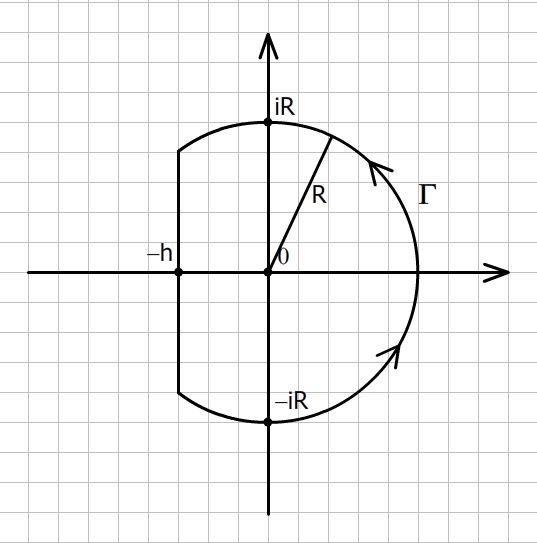
\includegraphics[scale=0.7]{Lecture04_Gamma}~\\
		(Рис. 1)
	\end{center}
	Значит, в $I(T): \ F(1+s)$ -- аналитична в области (по построению), $F_T(1+s)$ -- везде целая, $T^s$ -- целая (экспонента), $\displaystyle \frac{s}{R^2}$ -- целая, $\displaystyle \frac{1}{s}$ -- полюс порядка $1$ в нуле. Следовательно, по теореме Коши о вычетах 
	$$I(T) = \left(F(1)-F_T(1)\right)T^0 = F(1)-F_T(1).$$
\end{pf}

\begin{lemma} \label{l4_lm13}~\\
	При $\displaystyle \sigma = \Re(s)>0: \quad \lvert F(1+s)-F_T(1+s) \rvert \leq A\frac{T^{-\sigma}}{\sigma}$;\\
	при $\displaystyle \sigma = \Re(s)<0: \quad \lvert F_T(1+s) \rvert \leq A\frac{T^{-\sigma}}{-\sigma}$,\\
	где $A$ такое, что $\displaystyle \left| \frac{\psi(x)}{x}-1 \right| \leq A$ при $x \geq 1$.
\end{lemma}
\begin{pf}~\\
	$\displaystyle \sigma>0: \quad \left| F(1+s)-F_T(1+s) \right| = \left| \int_T^{+\infty}\frac{\psi(x)-x}{x^{2+s}}dx \right| \leq A\int_T^{+\infty}\frac{dx}{x^{1+\sigma}} = A\frac{T^{-\sigma}}{\sigma}$;\\
	$\displaystyle \sigma<0: \quad \left| F_T(1+s) \right| = \left| \int_1^T\frac{\psi(x)-x}{x^{2+s}}dx \right| \leq A\int_1^T\frac{dx}{x^{1+\sigma}} = A\frac{T^{-\sigma}}{-\sigma}$.
\end{pf}